\documentclass[12pt,a4paper]{article}
\usepackage[T1]{fontenc}
\usepackage[utf8]{inputenc}
\usepackage{lmodern}
\usepackage[margin=20mm]{geometry}
\usepackage{microtype}
\usepackage{graphicx}
\usepackage{booktabs,array}
\usepackage{pdflscape}
\usepackage{caption}
\usepackage[authoryear,round]{natbib}
\usepackage{xcolor}
\definecolor{linkblue}{RGB}{25,70,110}
\usepackage[colorlinks=true,allcolors=linkblue,
  pdftitle={Point-star astrometry across a fisheye field},
  pdfauthor={Peter Thejll}]{hyperref}
\graphicspath{{figures/}}
\captionsetup{font=small,labelfont=bf,skip=6pt,hypcap=false}
\setlength{\parindent}{0pt}
\setlength{\parskip}{5pt}
\setlength{\bibsep}{2pt}
\newcommand{\px}{\,\mathrm{px}}

\begin{document}
\begin{center}
  {\LARGE\bfseries Point-star astrometry across a fisheye field\par}
  \vspace{4pt}
  {\large A Barghini-model feasibility result\par}
  \vspace{5pt}
  Peter Thejll \quad\textbullet\quad 13 September 2026
\end{center}

An untrailed $1569\times1444$-pixel Milky Way image yields 3,688 measured
sources and 3,653 fitted catalogue associations. The root-mean-square (RMS)
positional residual is $0.398\px$, with median $0.249\px$.
Figure~\ref{fig:overlay} shows the agreement across the observed sky;
Figure~\ref{fig:residuals} resolves the remaining discrepancies.

\begin{center}
  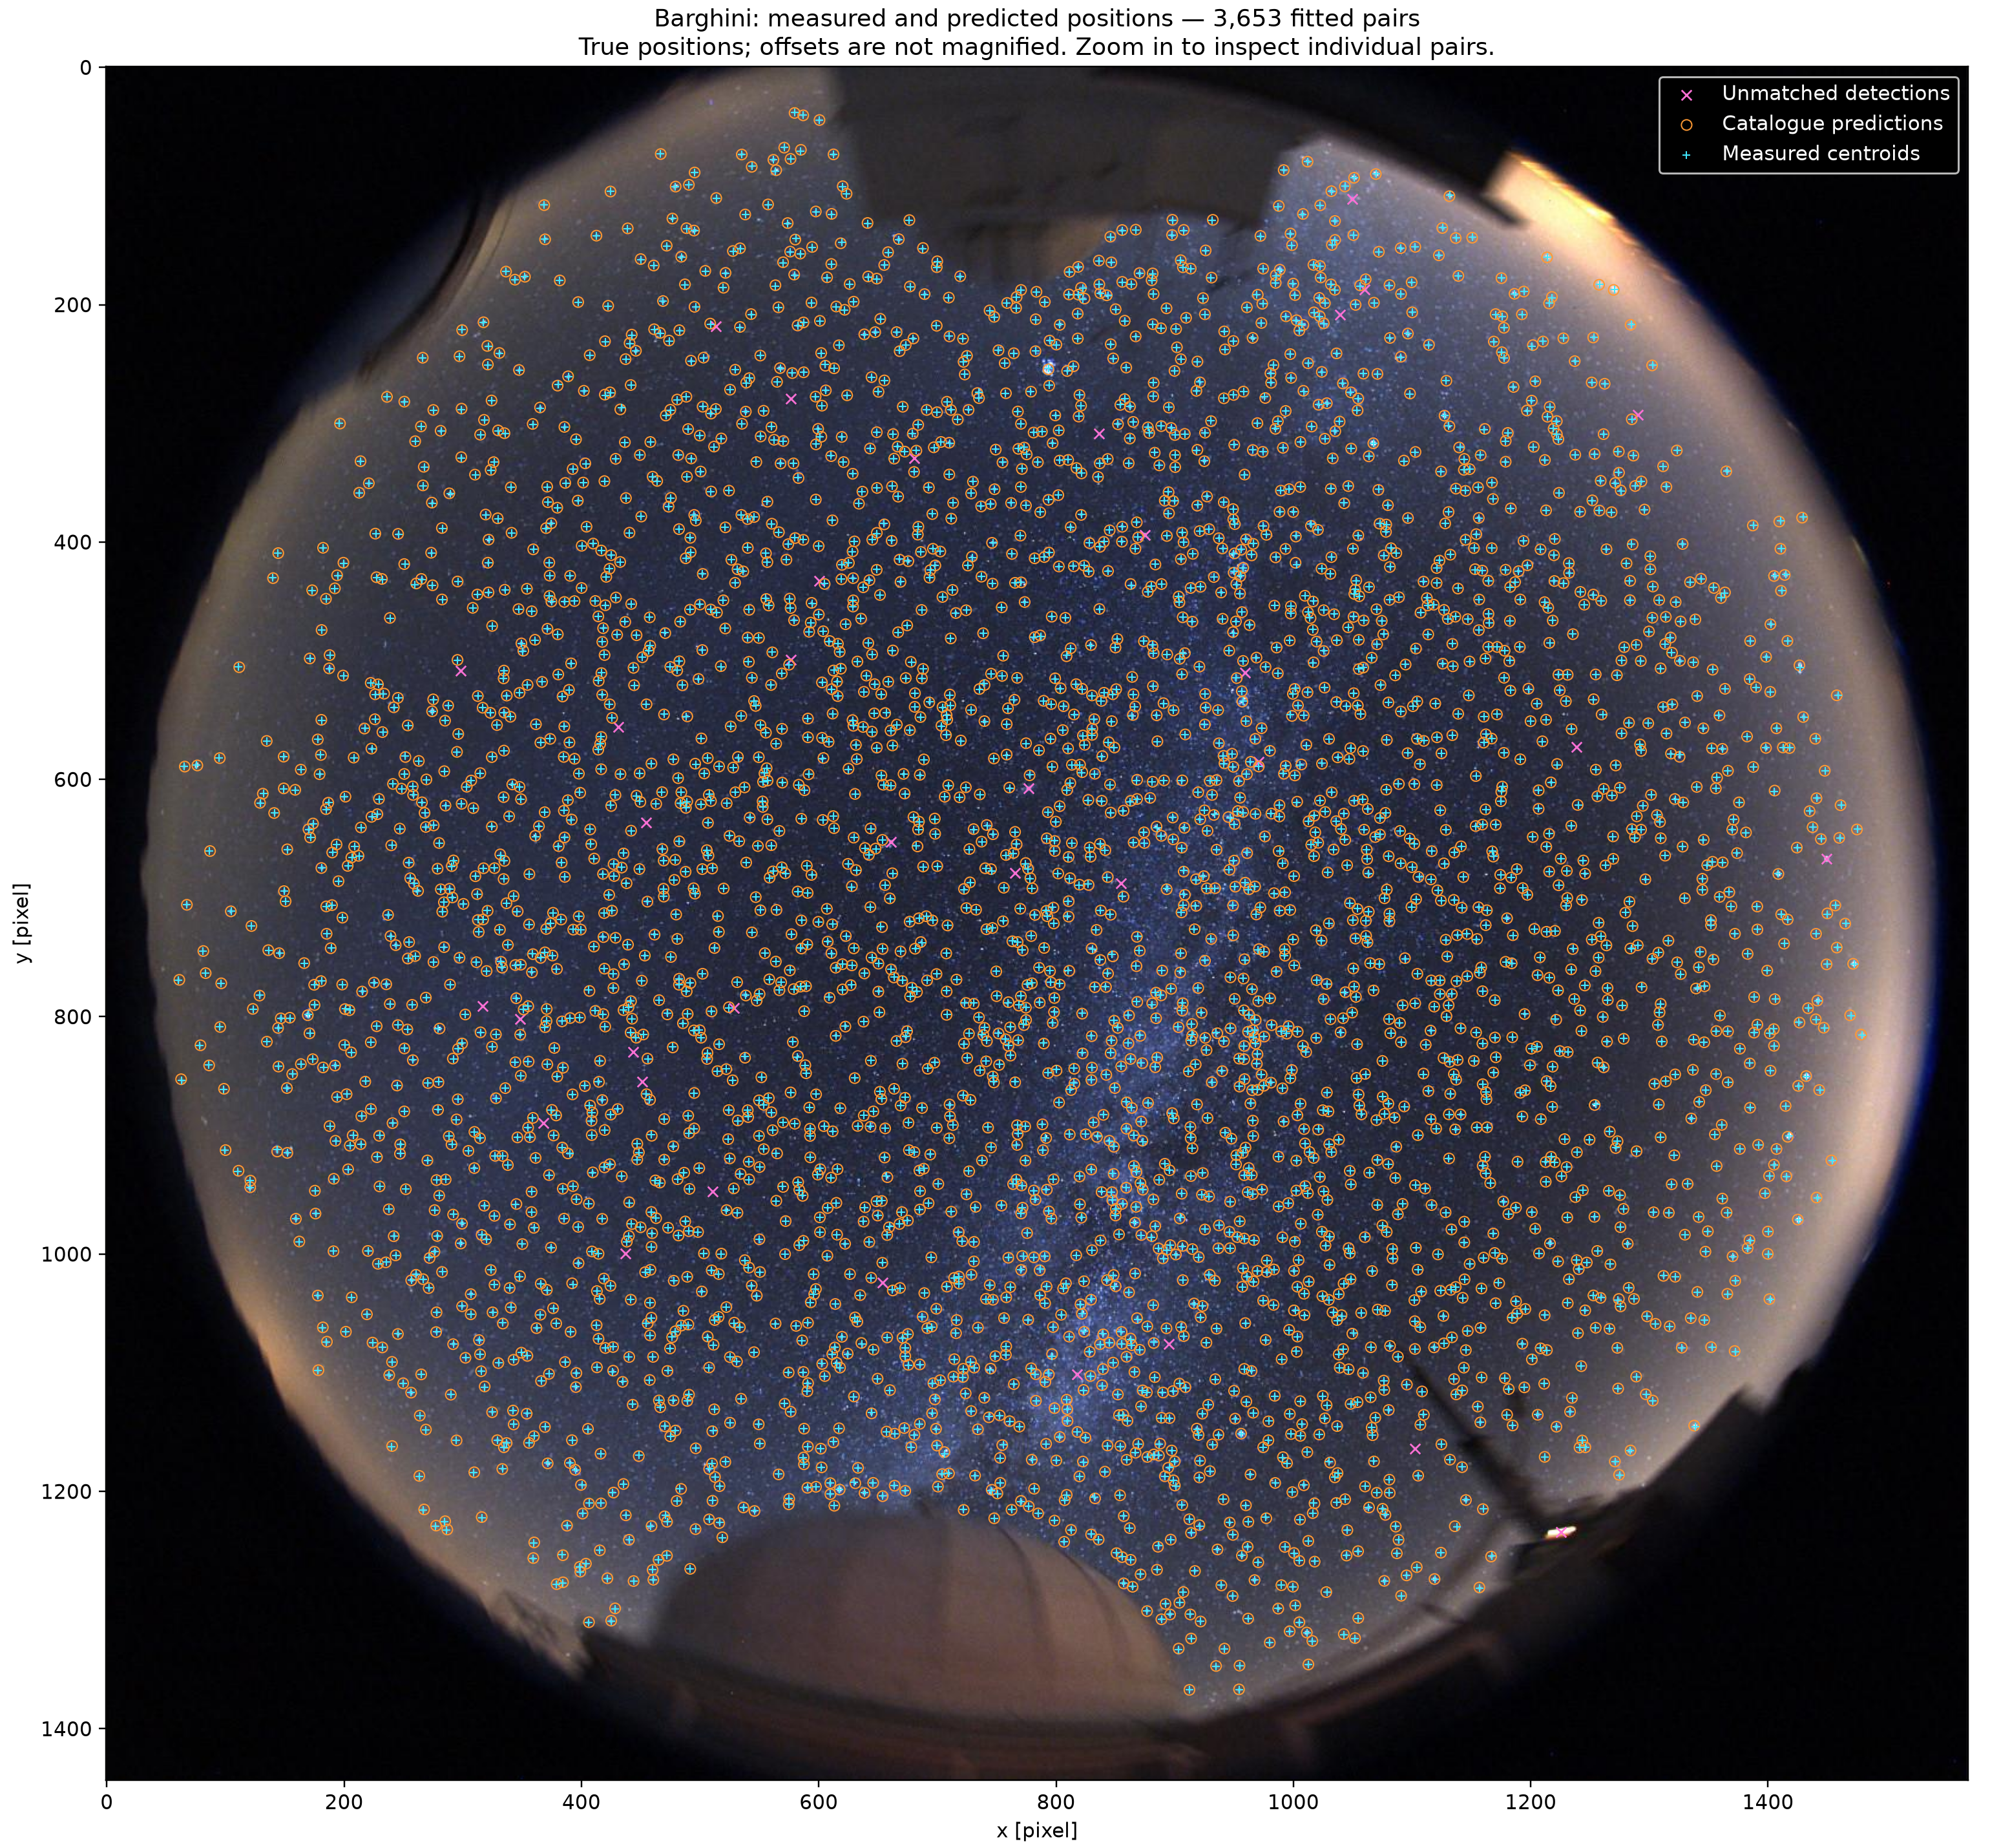
\includegraphics[width=.98\linewidth]{astrometry_overlay.png}
  \captionof{figure}{Measured centroids (cyan crosses) and catalogue positions
  projected through the fitted Barghini model (orange circles), for all 3,653
  fitted pairs. Pink crosses mark 35 unmatched detections. Coordinates and
  separations are displayed at their true image positions; no cosmetic shifts
  or residual magnification are applied. The full-resolution PDF supports
  inspection by zooming.}
  \label{fig:overlay}
\end{center}

\clearpage
\begin{landscape}
{\Large\bfseries Centre-to-edge behaviour\par}
\vspace{3pt}
\begin{center}
  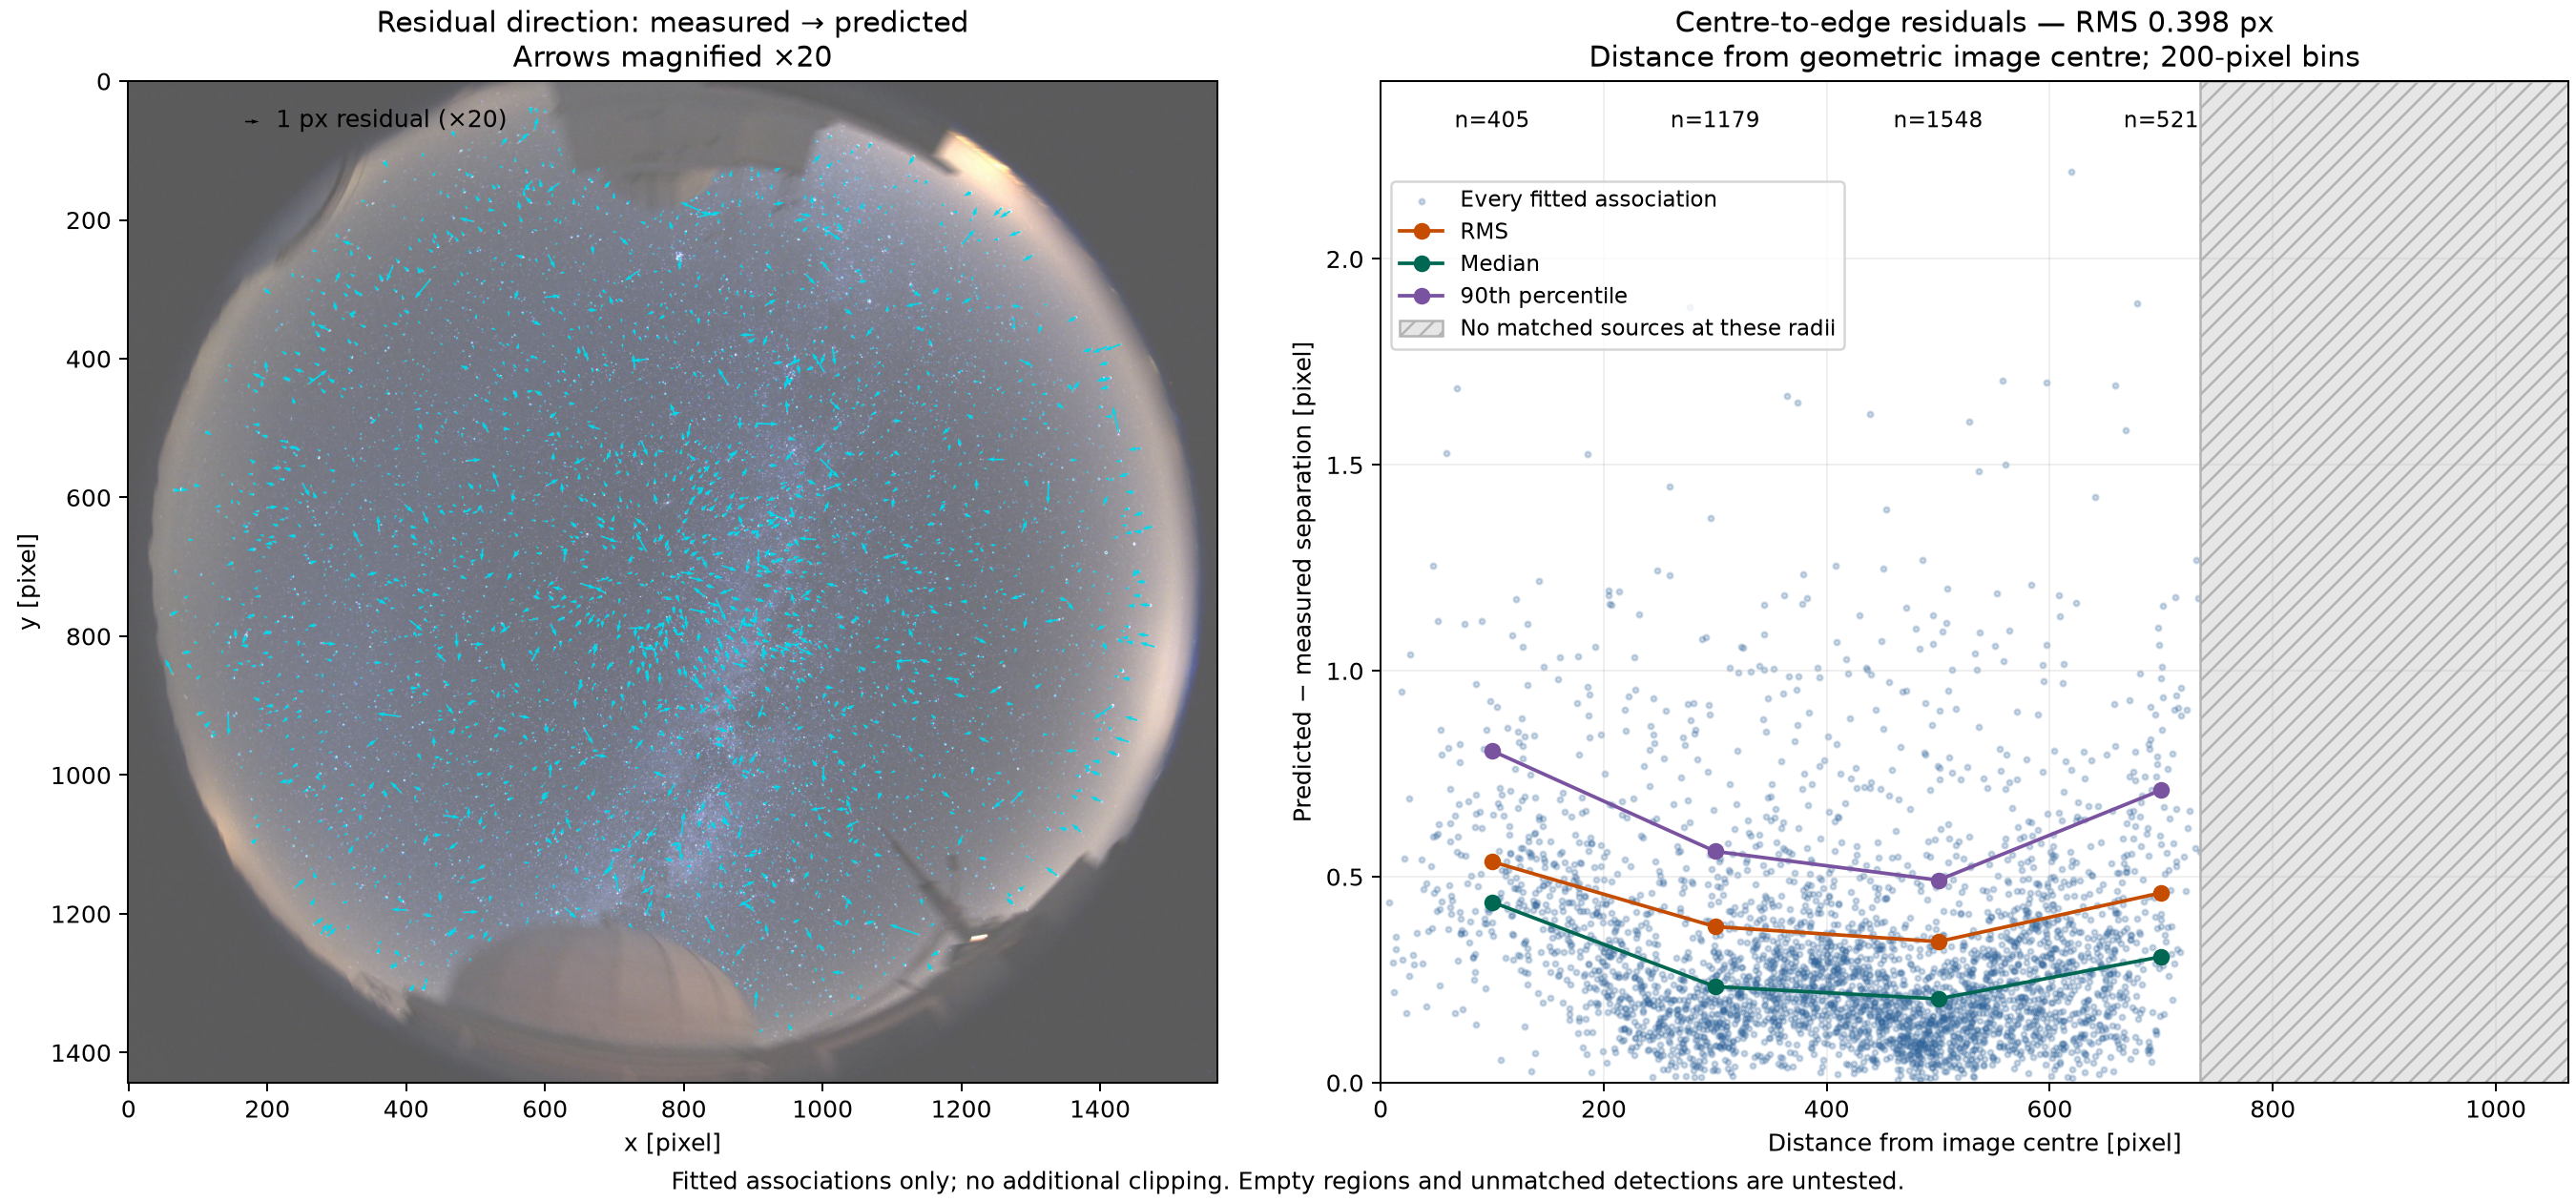
\includegraphics[width=\linewidth]{astrometry_residuals.png}
  \captionof{figure}{Left: vectors from measured to predicted positions,
  magnified $\times20$ solely for visibility. Right: separation for every fitted
  association, with RMS, median and 90th percentile in 200-pixel annuli about
  the geometric image centre. The hatched region has no matched sources.
  No additional residual clipping is applied. These diagnostics describe
  fitted associations, not independent validation.}
  \label{fig:residuals}
\end{center}
The outer band shows a modest RMS rise, without progressive edge divergence
among the matched sources. Small coherent residual patterns remain visible.
Any future correction must be made through the astrometric model and its
exported coordinates; plotting must preserve the resulting discrepancies.
\end{landscape}

\section*{Method and quantitative result}
Centroids are measured directly from the image after local background
subtraction. Growing measurement windows retain broad and saturated sources.
A blind \href{https://github.com/esa/tetra3}{tetra3} pattern match supplies
11 initial star associations from a small patch. Progressive matching against
the frozen Tycho-2 catalogue, supplemented with bright Hipparcos stars, then
expands the fitted field. The global projection uses the independent $O/Z$
parametrisation of \citet{barghini2019}, equations (5), (6) and (11), with
the inherited fish-eye transform discussed on page~\pageref{sec:lineage}:
\[
  u(r_O)=V r_O+S\bigl[\exp(D r_O)-1\bigr],
\]
where $r_O$ is distance from the optical centre. The diagnostic radius in
Table~\ref{tab:radial} is instead measured from the geometric image centre,
$(784.0,721.5)$ pixels.

\begin{center}
\captionof{table}{Residuals for all fitted associations in each image-centred
annulus. Radial bias is the mean signed component of predicted minus measured
position, positive outwards. All residual columns are in pixels.}
\label{tab:radial}
\smallskip
\begin{tabular}{@{}rrrrrr@{}}
\toprule
Radius [px] & Stars & RMS & Median & 90th pct. & Radial bias \\
\midrule
0--200   & 405   & 0.536 & 0.439 & 0.806 & $+0.329$ \\
200--400 & 1,179 & 0.379 & 0.233 & 0.562 & $-0.068$ \\
400--600 & 1,548 & 0.343 & 0.204 & 0.492 & $+0.015$ \\
600--800 & 521   & 0.461 & 0.306 & 0.711 & $-0.040$ \\
\bottomrule
\end{tabular}
\end{center}

\textbf{Interpretation.}
The largest fitted separation is $2.211\px$; the outermost matched source
is at radius $734.75\px$, so the last populated annulus is only partly
sampled. The inner-band outward bias of $0.329\px$ shows that systematic
structure remains. All sources were available for fitting, with no stars
withheld. Associations were selected with a three-pixel gate before the
final fit. Unmatched sources and unsampled regions have no evaluated
star-pair residual. The results therefore establish the feasibility of this
full-field fit, with conditional fit residuals rather than an independent
accuracy or completeness estimate. Observation-epoch propagation, atmospheric
refraction and terrestrial orientation are outside this experiment.

\textbf{Comparison and next steps.}
In the recorded, time-bounded comparison, direct whole-image
\texttt{solve-field} attempts were unsolved. On a $260\times260$-pixel crop,
the same measured dots gave $0.390\px$ RMS with third-order SIP distortion,
against Barghini's $0.406\px$ on the same 195 stars. This supports a benefit
in field coverage while demonstrating comparable local precision.
Further work should test other images and lenses, and evaluate a bright-star
supplement plus Gaia DR3/DR4 in place of Tycho, with epoch propagation.

\clearpage
\section*{Scientific lineage and scope of this implementation}
\label{sec:lineage}
\citet{barghini2019} explicitly place their method within earlier fireball-camera
astrometry in their Section~2. The principal development is:

\textbf{Ceplecha (1987).}
The empirical radial description $z=U+Vr+S\exp(Dr)$ accounts for the strong
change in image scale towards the horizon. Barghini and colleagues credit
\citet{ceplecha1987} with this starting point for the all-sky model.

\textbf{Borovi\v{c}ka (1992).}
The subsequent formulation separates projection coordinates about the optical
axis from horizontal celestial coordinates and gives the constrained radial
law $u=Vr+S[\exp(Dr)-1]$ \citep{borovicka1992}. This eight-parameter model is
also reproduced explicitly in Section~1.2 of \citet{borovicka1995}.

\textbf{Borovi\v{c}ka, Spurn\'y and Kecl\'ikov\'a (1995).}
Their tests on guided all-sky photographs exposed systematic near-horizon
errors in the preceding model. They introduced an additional exponential
term in squared radius and corrections for plate inclination
\citep{borovicka1995}. Their Figures~2--3 demonstrate the same diagnostic
principle used here: examine residuals across the field and correct the
astrometric transformation when the evidence requires it.

\textbf{Barghini and colleagues (2019).}
Their Sections~4.2--5 identify strong coupling between optical-centre
coordinates and the angular offset to the zenith. Replacing the latter by
explicit detector coordinates of the zenith yields the $O/Z$ parameterisation
used here. They also describe initialisation from meridian crossings,
progressive source association and centroiding tests \citep{barghini2019}.
Thus the radial projection has a clear lineage, while the 2019 work improves
its parameterisation and practical calibration.

\textbf{What this experiment adopts.}
Our single-image solver combines the analytical $O/Z$ model with its own
dot finder, tetra3 bootstrap and robust fit. It does not reproduce the paper's
multi-epoch meridian-crossing initialisation: $Z$ is a fixed celestial reference
direction here, with no inferred local zenith. The extra 1995 correction terms
and Barghini's Section~6.4 tabulated systematic corrections are also absent.
The remaining residuals are displayed faithfully; any added calibration must
be part of the sky--pixel mapping and saved coordinates.

\textbf{Reproducibility.}
The \href{https://github.com/hotblack43/WIDE-FIELD-SOLVER}{private
\texttt{WIDE-FIELD-SOLVER} repository} preserves the original solver at
\href{https://github.com/hotblack43/WIDE-FIELD-SOLVER/releases/tag/v0.1.0}{\texttt{v0.1.0}}.
The diagnostics retain the same camera and coordinates. Both figures are
included unchanged. The photograph's original attribution and redistribution
terms are undocumented; this report is for private research use.

{\small
\bibliographystyle{plainnat}
\bibliography{references}
}
\end{document}
